\chapter{Experiments}
In the previous chapter we have outlined all the important steps in the process of constructing Vector 
Space Models, and listed all major approaches that we thought to be important for the task of Word 
Sense Disambiguation. There are certainly many other approaches that are employing VSM in some CL 
or NLP task, but because their domain of application is not relevant for the task of interest they where not 
mentioned here. This chapter is devoted to describing the full methodology behind the experiments 
performed in this thesis as well as how this methodology stems from previous approaches in VSM, 
in all the relevant phases of the process. First we will describe the resource that WSD was performed on, 
Prague Dependency Treebank, which will be followed with data preprocessing section. In the section 
after we will describe all the models implemented for the WSD task. After that the evaluation rationale 
will be presented. All experiments were performed on the principle: one model-- one experiment. In the 
final sections of this chapter results of experiments with the baseline random guessing scores will be 
 presented.


\section{The resource}
Prague Dependency Treebank (PDT) is  project that stemmed from work of a group of Czech linguists 
(Institute of Formal and Applied Linguistics\footnote{http://ufal.ms.mff.cuni.cz/}, Institute of Theoretical 
and Computational  Linguistics\footnote{http://utkl.ff.cuni.cz/}) from Charles 
University\footnote{http://www.cuni.cz/} in Prague and Masaryk 
University\footnote{http://www.muni.cz/}  in Brno. PDT was  inspired by the research resulting from the 
Penn Treebank\footnote{http://www.cis.upenn.edu/~treebank/} project. 

PDT was generated in two major phases. In the first phase (1996--2000), the morphological and syntactic analytic  layers of annotation have been completed along with the preview of tectogrammatical layer annotation available as  PDT 1.0. During the second phase (2000--2004), the tectogrammatical layer of annotation was completed and PDT 2.0 was done.
\\The structure of Prague Dependency Treebank (PDT) consists of three layers:
\begin{itemize}
\item morphological layer (lowest)-- full morphological annotation
\item analytic  layer (middle) -- superficial (surface) syntactic annotation using dependency treebank; level conceptually close to the syntactic annotation used in the Penn Treebank 
\item tectogrammatical layer (highest) -- level of linguistic meaning
\end{itemize}
In our experiments we were using as a resource PDT1.0 version, instead of PDT2.0. Frequencies for each layer in PDT1.0. are given in the table below:
\begin{table}[h!]
\begin{center}
	\begin{tabular}{ l  c  | c c }
   	&    & \# of tokens & \# of sentences \\
	\hline                       
	& morphological (total) & 1,725,242 & 111,175\\
	& syntactic--analytic (total) & 1,507,333 & 98,263 \\
  	& tectogrammatical (portion) & 3,490 &  203 \\
	& morphological and syntactic--analytic & 1,255,590 & 81,614 \\
	\end{tabular}
\end{center}
\caption{Frequencies of tags for every layer in PDT1.0.}
\end{table}
\\\\\\\\
\textbf{Text Sources}
\\\\The text material that was annotated in PDT contains samples from the following sources:
\begin{itemize}
\item Lidov\'e noviny\footnote{http://www.lidovenoviny.cz/} (daily newspapers), 1991, 1994, 1995
\item Mlad\'a fronta Dnes\footnote{http://www.idnes.cz/} (daily newspapers), 1992
\item Ceskomoravsk\'y Profit (business weekly), 1994
\item Vesm\'ir (scientific magazine), Academia Publishers, 1992, 1993
\end{itemize}

\subsection{Polysemous words}\label{pdt}
Czech language is the typical representative of inflectionally rich free--word--order language\footnote{http://www.czech--language.cz/index.php}, which surely doesn't have a favorable influence on the number of polysemous words in Czech language. From the training set that represents approximately 9/10 of the whole PDT1.0 we present in the table below the number of words that have more than one meaning. In the left column is given the number of meanings, and in the right column the number of words that take that number of meanings. For instance, the eight row informs us that there are two words that take 8 different meanings in the training set.
\begin{table}[h!]
\begin{center}
	\begin{tabular}{ c  c |  c }
   	&   \# of meanings & \# of types \\
\hline  
 & 2 & 329  \\
 & 3 & 37  \\
 & 4 & 20  \\
 & 5 & 6  \\
 & 6 & 4  \\
 & 7 & 4  \\
 & 8 & 5  \\
 & 9 & 3  \\
 & 10 & 3  \\
\hline  
& &Total =411\\  
 	\end{tabular}
\end{center}
\caption{Number of types with multiple meanings in the training set}
\end{table}
Another interesting ratio to be taken into account is the number 



\subsection{Why PDT1 instead of PDT2?}
The question from the title of the section is indeed a perfectly valid and reasonable question indeed, for 
any type of research-- why use an older version of a resource, when there is a newer, more complete 
version of the same resource?  

To answer this question we must go back to the task that is in focus of this research. For the WSD task the 
important feature of the text on which the system is trained and tested on is that every different meaning of a 
word is marked orthographically different. This information that could be extracted both from PDT1.0 and 
PDT2.0, therefore for the WSD task one resource is as much sufficiant as the other one. The only 
difference between the two treebanks is that PDT2.0 contains additionally the tectogramaticall layer, that 
was not used in this research.  

When building(training) Vector Space Models, a researcher might want to include POS information with 
every tag. This was not done in our experiments but it was always an option supported by the resource, 
because like previously mentioned, PDT1.0 is fully annotated on the syntactic level. 
\\On top of these reasons, another incentive that made us decide for PDT1.0 is that it essencially 
represents a light--wight version of PDT2.0, encoded in Standard Generalized Markup Language 
(SGML\footnote{http://www.w3.org/MarkUp/SGML/}), which made it easier to handle during the 
preprocessing stage.

\section{Preprocessing}
The preprocessing phase involves several several sub--stages. As we have described theoretical approaches to these steps in length in previous chapters, we have decided to explain all the preprocessing steps performed in experiments in this chapter. Preprocessing involves following sequential steps: text extraction from PDT files along with relevant annotation, text normalization, stemming and filtering. 
\\\\  \textbf{Text extraction}

Text used during training and testing phase of VSM was extracted from PDT files and put into a single file. 
In order to make the implementation applicable for other resources other than PDT we have made a 
design decision that the implementation uses this single file as its input. Apart from the single--meaning 
words, the system extracts multiple meaning words, and represents differently each separate meaning. In 
PDT1.0 if a word has multiple meanings, meaning of that word is given in a separate tag, in the following format: 
\textit{word--index\_number\_of\_meaning}. Index number increments as the word has more meanings.

Therefore, the annotation step in this case was simplified: \textit{every multiple--meaning word was 
represented with its orthographic representation meaning in context}, which was simply extracted from 
the Treebank. An example of a sentence extracted from PDT is given below:
\begin{examples}
\item Krumbachov\'a pr\'aci p\^rijmout--2 podle--2 vlastn\'i--1 slov " v--1 hodin\^e dvan\'act\'e ".
\glt \textit{ Krumbach has accepted the work " in the last minute" .} 
\end{examples}
Word's meaning in context was given as it was represented in PDT.
\\\\  \textbf{Text normalization}

Czech language has spelling variants-- words that are orthographically slightly different but are actually 
identical on every other level of analysis, for example words like \textit{abch\'azsk\'a}  and 
\textit{abchazsk\'a}. Many foreign names have variant spellings, especially in marking the vowel length. 
Spelling variants should not be counted as different types so it was therefore decided to normalize all 
characters with diacritics marking the vowel length into characters without them. 
\\As a measure of normalization that would reduce distributional sparsity of words all words were 
lowercased. Punctuation marks were also filtered from the entire corpus, so that the models could be 
trained on terms only. 
\\\\  \textbf{Stemming}

Stemming process was detailed in the chapter\ref{linguisticPreprocessing}, as well as how it is different 
from lemmatization. To re--iterate: lemmatization is more precise than stemming because it picks up 
lexical variants that are not orthographically similar to the stem. At the same time it is much harder to 
implement than a stemmer, because it requires utilization of a lexicon. 

Although a good lemmatizer was built at 
UFAL\footnote{http://ufal.mff.cuni.cz/pdt/Morphology\_and\_Tagging/Morphology/index.html}, it was not 
used 
in this system. During preliminar experiments with cosine-weighted co-occurrence matrix it was observed 
that the improvement in precision when applying lemmatizer over stemmer is not  significant. It was 
therefore
assumed that precision would not be improved in other models experimented with as well. 
A stemmer built for the Czech language made at University of 
Neuchatel\footnote{http://members.unine.ch/jacques.savoy/clef/CzechStemmerLight.txt} was used in 
preprocessing 
phase.  An example of text that 
was extracted, normalized and stemmed is given below:
\begin{examples}
\item krumbach prak p\^rijmout--2 podle--2 vlastni--1 slov " v--1 hodin dvanact ". 
\glt \textit{  Krumbach has accepted the work " in the last minute"  .} 
\end{examples}
Stemming was left as an optional measure in order to observe whether it improves the precision of algorithm.
\\\\  \textbf{Word Filtering}
\\Two effective filtering criteria were applied (optionally) in our experiments for the purpose of reducing the sparsity of vectors and improving overall precision: POS and low frequency counts. A list of Czech stop words was compiled(Apendix A) in order to filter out words that belong to closed grammatical classes. Both types of filtering were experimented with, in order to observe how their tunning influences the overall precision of system.

\section{Train and test sets}\label{trainTestSet}

After extracting the text from PDT and optional preprocessing normalization performed on text, text's 
sentences are randomized and split into 3 separate files: $train, testDev, testFinal$. Training set holds 
85\% of the number of sentences in the whole set, while $testDev$ holds about 5\% and $testFinal$ 
about 10\%. First test file 
($testDev$) is used to evaluate during training phase, while the second ($ testFinal$) is used for 
evaluation in the testing phase. 

Below is given an overview of the number of types and tokens for each of these files, before and after 
preprocessing applied to them:

\begin{table}[h!]
\begin{tabular}{ l | c c | c c | c c|}
& \multicolumn{2}{|c}{train set} & \multicolumn{2}{|c}{test devel set} & \multicolumn{2}{|c|}{final test set} \\
   &  \#types & \#tokens  &  \#types & \#tokens  &  \#types & \#tokens \\
  \hline                       
  no preprocessing & 114720 & 1080400 & 10439 & 32105 & 27626 & 113330\\
  merge variants & 114696 & 1079851 & 10418 &  32033 & 27530 &112678\\
  stemming & 62063 & 1050948 & 7699 & 29891 & 18122 & 105912\\
\end{tabular}
\caption{Influence of the preprocessing method on the size of training and test sets}
\end{table}
We can observe that stemming reduces the vocabulary size much more than merging 
lexical variants. This fact will reflect on the precision in the evaluation phase. 

\section{Document size}
After preprocessing phase, the next is to build the term--document matrix. This step is generalized for all models we will be training. This is because the term--document matrix is a simple frequency matrix, and (optional) normalization of frequency counts or dimensionality reduction takes place in the next phase. Crucial property of this phase is the size of the document in the term--document. Previous approaches were described on the use of context, ranging from word--level to paragraph--level. Document size used in the following experiments will be: 
\begin{itemize}
\item five sentence paragraph
\item three sentence paragraph
\item one sentence paragraph
\item three neighboring words of preceding and succeeding context
\item two neighboring words of preceding and succeeding context
\item one neighboring word of preceding and succeeding context
\end{itemize}
To further clarify what exactly do last three items in the list mean, we will point out that the since the task
at hand is disambiguation of polysemous words. Therefore, polysemous meanings should be in focus of
every document. We have decided to conduct experiments by partioning sentences into fragments where 
in the center of every such fragment is a polysemous meaning, surrounded by symmetrical window 
length of varying size. An example is given for a one neighboring word of preceding and succeeding context. For a sentence:
\begin{examples}
\item Krumbachov\'a pr\'aci p\^rijmout--2 podle--2 vlastn\'i--1 slov " v--1 hodin\^e dvan\'act\'e ".
\glt \textit{  Krumbach has accepted the work " in the last minute" .}
\end{examples}
, corresponding fragments extracted from it are:
\begin{examples}
\item pr\'aci p\^rijmout--2 podle--2
\item p\^rijmout--2 podle--2 vlastn\'i--1
\item podle--2 vlastn\'i--1 slov
\item slov v--1 hodin\^e
\end{examples}
Although this fragmentation increases the volume of documents we believed that centering somehow
documents around polysemous encounters will help train the model better. The rationale behind that decision was that this was an assumption that this way the model will become ''more sensitive" to assigning  correct meanings to their rightful contexts. 

Choice of document size during model training is one of the crucial features of VSM, and can very much 
influence the results of the model's performance, through the size of vocabulary. Size of vocabulary is 
influenced by 
preprocessing method applied as well the size of the document. Below is given a table that shows how 
the choice of document size influences the size of vocabulary, for the corpus that was not preprocessed. 

\begin{table}[h!]
\begin{tabular}{ l | c | c c |c c}\label{docSize}
			& \#index  &  ambiguous  words && other words \\
 document size & documents & \#types & \#tokens & \#types & \#tokens \\
\hline
5 sentences & 15732 & 3513 & 4721 & 128676 & 1155781\\
3 sentences & 26220 & 3334 & 4417 & 129618 & 1166559\\
1 sentence & 78660 & 2116 & 2660 & 130620 & 1216412\\
3+3 & 231673 & 2116 & 2660 & 105225 & 1433731\\
2+2 & 231673 & 2116 & 2660 & 94018 & 1088417\\
1+1 & 231673 & 2116 & 2660 & 70772 & 700799\\
\end{tabular}
\caption{Influence of document size on the volume of vocabulary}
\end{table}

With the word--level document size we can observe that number of types is smaller than in sentence
--level documents. This is due to existing gaps between documents in matrix with word--type document.
Number of tokens  can be bigger which we see in the case of 3+3 document size, because in some 
places, where two occurrences of ambiguous words stand next to each other, there will be an overlap
which will be counted. 

\section{Normalization of the frequency counts and dimensionality reduction}
Normalizing the frequency counts was done in two ways in experiments: the traditional TF--IDF weighting, and the enthropy--based weighting as prescribed in LSA. To re--iterate the formulas again:
 \begin{center}
\begin{equation}\large{f_{ij} = TF_{ij} \cdot DF_{i} \cdot S_{j}}
\end{equation}
\end{center}
,where $TF_{ij}$  is the frequency of term \textit{i} in document \textit{j}, $DF_{i}$ is some function of the number of documents term i occurs in (DF for \textit{document frequency}), and $S_{j}$ is a normalizing factor, usually dependent on the length of document(s for scaling).
DF is usually computed as:
\begin{center}\large{
\begin{equation}IDF = log \frac{D}{DF_{i}}
\end{equation}
}
\end{center}
, where D is the total number of documents in the whole corpus. 
%\todo{
%++Keyword Density Values
%\begin{large}
%$ KD_{i} = \frac{tf_{i}}{L_{i}}  $
%\end{large}
%}
\\\\  
Another frequency weighting performed was the entropy--based weighting as given in the formula below:
\begin{center}\large
\begin{equation}E_{ij}=1+  \frac{\sum_{j}{P_{ij}log P_{ij}}}{logD}
\end{equation}
\end{center}
where \textit{D} is the total number of documents in the collection. $P_{ij}$ is given with a formula
\begin{equation}\large{P_{ij} = \frac{TF_{ij}}{f_{i}}} \end{equation}
where $TF_{ij}$ is the frequency of term $i$ in document $j$ and $f_{i}$ is the frequency of term \textit{i} in the whole document collection.

Another model that was experimented with is created through the use of dimensionality reduction 
technique-- Random Indexing. Frequencies counts of its term--document matrix were not normalized, 
due to the nature of its generation. Detail description of RI is given in chapter\ref{RI}. What should be 
restated is that:
\begin{itemize}
\item It builds term vectors by adding pseudo--random vectors assigned to documents in the corpus.
\item It uses fixed dimensionality for both term and document vectors, which means that new data do not 
increase the dimensionality of the vectors.
\item It uses implicit dimensionality reduction, since the fixed dimensionality is
much lower than the number of contexts in the data. Producing
context vectors with RI is only $O(wr)$, since the method is not reliant on the
initial construction of the co-occurrence matrix.
\item It is incremental, which means that the context vectors can be used for similarity
computations even after just a few examples have been encountered.
\end{itemize}
More details on RI can be found in Chapter\ref{RI}. 

The two approaches to weighting the co--occurrence matrix(TF--IDF and PMI) and one approach to 
dimensionality reduction (RI) are considered as fundamentally different. That is why the experiments are organized around these models, with other 
parameters like preprocessing, document size, and evaluation context size and number of word 
meanings threshold used in the evaluation(both explained in following sections) are changed to investigate how they influence the overall performance. 

\section{Evaluation context size} 
After the co-occurrence matrix is built and frequencies of its elements are normalized with some 
value (TF--IDF or PMI), or the matrix's dimensionality is reduced (RI) our model is ready to be tested out.
This means that now for every word in the dictionary we have a vector that is in a way its representation.
A unique methodology is then applied for each model in order to calculate the measure of appropriateness for a current word meaning against the context it is found in. Size of the context around the current meaning in question is experimented with and in our experiments takes values from 1 to 7, to determine the influence of symmetric context size on the overall accuracy. 
Evaluation context size is the number of words taken from preceding and succeeding context of the 
occurrence of ambiguous word. For instance, for the sentence:
\begin{examples}
\item Krumbachov\'a pr\'aci p\^rijmout--2 podle--2 vlastn\'i--1 slov " v--1 hodin\^e dvan\'act\'e ".
\glt \textit{ Krumbach has accepted the work " in the last minute"  .}
\end{examples}
, corresponding contexts for the evaluation context size set to 1 extracted from it are:
\begin{examples}
\item p\^rijmout--2 : pr\'aci  podle--2
\item  podle--2: p\^rijmout--2 vlastn\'i--1
\item podle--2 slov
\item slov  hodin\^e
\end{examples}


In the implementation level, the way the most appropriate meaning for a context is calculated in two passes:
\begin{itemize}
\item The test set is traversed, in order to extract all the contexts for all the polysemous words 
encountered  in testing.
\item Extracted contexts are traversed, and for every different meaning the appropriateness for that 
word meaning in context is calculated. The meaning that has the highest score is selected as the 
true meaning by the system.
\end{itemize}  
Two things here are of importance: the way context vectors is built, and the way distance between context vector and meaning vector is calculated. Context vector in all cases (TF--IDF, PMI and RI) is 
built by superposition of all the term vectors constituting that context. If the term was not encountered 
during training it is skipped. If context vector does not have any terms inside it then that context is skipped during evaluation. This means a difference in size of vocabulary made in training can influence the number
of contexts being evaluated, and therefore the test set size. 

Distance between context and 
meaning vector is calculated as a cosine distance in all cases.

To repeat, cosine distance is  the angle between two vectors $\vec x$ and $\vec y$, defined as:
\begin{center}
\large{
\begin{equation}sim_{COS}(\vec x ,\vec y) =  \frac{\sum_{k=1}^n x_{i}y_{i} }{\sqrt []{\sum_{k=1}^n x_{i}^{2}} \sqrt []{\sum_{k=1}^n y_{i}^{2}}} 
\end{equation} 
}
\end{center}

\section{Evaluation metrics and baselines}
In this section evaluation metrics and baselines used in this research will be presented, employed for 
\textit{in vitro} evaluation of WSD systems (Navigli 2009). The evaluation the WSD system as a module 
embedded in applications (called \textit{in vivo} or \textit{end-to-end} evaluation) was not conducted 
in this research.  
\\\\
All sentences extracted from the PDT and annotated to distinguish different meanings of polysemous
words are divided into three sets (files): training, test development, and test final. Training takes about
9/10 of the entire set, while the rest is distributed evenly between two test sets. During the training 
phase the model is trained on the training set, and evaluated on the test development set. In the evaluation
phase training and test development sets are merged, the model is trained on them, and evaluated on the
final test set, which represents the unseen portion of data. This ensures an unbiased evaluation of every
model.
\\\\
Given the individual training and test sets \textit{coverage C} is defined as the percentage
of items in the test set for which the system provided a sense assignment:
\begin{equation}
\large{C=\frac{\#answers\_provided}{\#total\_answers\_to\_provide}=\frac{TP+FP}{TP+FP+FN}
}
\end{equation}
\\\\
If the systems provides an answer for every test instance then $C=1$.
The \textit{precision P} of a system is computed as the percentage of correct answers given by the 
system. If the model ''calculates the correct meaning" properly, $\#correct\_answers\_provided$ is 
incremented. The total number of answers given by the system is counted as well, and then precision 
is calculated as: 
\begin{equation}
\large{P=\frac{\#correct\_answers\_provided}{\#answers\_provided}=\frac{TP}{TP+FP}
}
\end{equation}
%TODO REMOVE TP, FP, FN BECAUSE THE DEFINITIONS ARE NOT THE SAME IN WSD
\\\\
Precision determines how good are the answers given by the system.
\textit{Recall R} is defined as the number of correct answers given by the automatic system
over the total number of answers to be given:
\begin{equation}
\large{
R=\frac{\#correct\_answers\_provided}{\#total\_answers\_to\_provide}=\frac{TP}{TP+FP+FN}
}
\end{equation}
\\\\
If the coverage of the system is absolute ($C=1$) then recall and precision will be equal. 
From these two values (precision and recall) an F--measure is calculated according to formula:
\begin{equation}
\large{
F-measure=\large{\frac{1}{\frac{\alpha}{P}+\frac{1-\alpha}{R}}}
}
\end{equation}
where $\alpha$ is the weight factor which in experiments performed here takes the value of 0.5, in order to give equal weights to both precision and recall. 
\\\\
\textbf{Baseline.}

As a baseline result, random guessing is calculated for every test set used in evaluation. Random baseline is the random choice of a sense from those available for each polysemous word $w_i$ . Random 
precision is calculated as:
\begin{equation}
\large{
RandomP=\frac{1}{n} \sum_{i=1}^{n}\frac{1}{Senses(w_i)}
}
\end{equation}
where $Senses(w_i)$ is the number of senses that a $w_i$ can have. 

\section{Tuning}
Number of meanings that polysemous words encountered in the corpus can vary from 1 to 8 meanings. The actual number of meanings follows Zipf's distribution, where ranks are the number of meanings word 
can take (1 to 8) and numbers are the number of polysemous words that take that number of meanings. 
To illustrate this with a simple example: number of words that take 2 meanings in PDT1.0 is 329. 
Full table is given in chapter\ref{pdt}. Below is given a plot to illustrate how meaning's counts and word 
types conform to the Zipfian distribution.

\begin{figure}[h!]
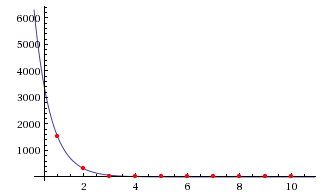
\includegraphics{img/meaningTypePlot.png}
\caption{Distrubution of number of polysemous types per number of meanings}
\end{figure}


Three types of experiments for each model were performed, in order to tune each model to achieve its 
best performance.
\subsection{Tuning preprocessing parameters}
Each of the preprocessing measures mentioned before 
(lowercasing, filtering words that belong to the closed class group, stemming and merging of lexical
variants in Czech language) was experimented against the different document size (5,3,1 sentence 
document and 3+3, 2+2, 1+1 words surrounding polysemous word) to determine for which parameters the model achieves the highest accuracy. These models were evaluated only for highly polysemous
words, at the fixed size of the evaluation context size. In  order to able to test how models really perform 
we train models only on highly polysemous words, the ones that have 6 or more meanings.  There are 19 
polysemous words in the test development set that can take 6 to 10 meanings.

\subsection{Tuning evaluation context size} 
When the best parameters for preprocessing and document size (in the term--document matrix) are 
discovered, the next tuning phase experiments with different sizes of Evaluation Context against these best 
paremeters. There are two motivations for this sequence of tuning experiments: first, the preprocessing
 and building the matrix come before matrix frequency normalization and evaluation. Second, after
the best parameters in the preprocessing stage are found, we can observe how this (best) model behaves 
with different sizes of context (from which the evaluation context vector is constructed). 

\subsection{Evaluation on polysemous words of different level } 
Words whose orthographic representation can take on a large number of meanings can be considered
as ''highly polysemous", while words that can take on a small number of meanings(like two or three) can 
be regarded as ''not highly polysemous". As explained, numbers of occurrences of polysemous words 
conform to the Zipfian distribution, which means that there is only a small number of highly polysemous
words. Therefore, when experimenting with such words test set is not overly large, but if other, less
polysemous words are included, the number of test set instances rise. The purpose of this experiment
is to investigate how do models handle more and less polysemous words. Ranges from 2 to 9 meanings per word
are taken into consideration.




\section{TF--IDF experiments}
As previously mentioned experiments are organized around 3 different different Vector Space Models, 
based on the weighting of the matrix elements or dimensionality reduction technique. Matrix reduction technique used for this model was TF--IDF (described in Chapter 6.5). For all models experiments were performed on every possible parameter, grouped into under the phase under which they were used:
\begin{itemize}
\item Tuning preprocessing parameters
\item Tuning evaluation context size
\item Evaluation on polysemous words of different level
\end{itemize}
These rounds are ordered sequentially in order to ensure best possible tuning for the model. Final step
is evaluation on  words with different number of meanings attached to them.

\subsection{Tuning preprocessing parameters}
First, no preprocessing method was applied on the train and test set. The size of the document in the term--document co-
ocurrence matrix was changed to observe the influence on the precision. A threshold number of meanings was set to 6, which means that other polysemous words that had less than 6 meanings encountered in training were dicareded for this test. Also an evaluation context size was fixed to 3. Document sizes that were
experimented with are: 5 sentence document, 3 sentence document, 1 sentence document, and 3+3, 2+2, 1+1 symmetric word windows around polysemous word.  
Random precision was calculated as well to serve as a baseline. 
Best results in all the tables are bolded. 
Precision (in \%) for every document size is presented in the tables below. First a sentence--level 
document size was experimented with. 
\begin{table}[h!]
\begin{tabular}{ l | c c | c c | c c | c}
   preprocessing &  5 sentences && 3 sentences && 1 sentence  && random\\
\hline
	& P  &  R & P  &  R & P  &  R &\\
\hline\hline
NO  & 93.65 & 100 & 94.23 & 100 & 93.84 & 100 & 29.38 \\
LOWCASE  & 97.56 & 100 & 95.71 & 100 & 95.28 & 100 & 7.3 \\
STEM  & 99.48 & 100 & 98.95 & 100 & 99.48 & 100 & 14.12 \\
MERGE  & 99.48 & 100 & 98.95 & 100 & 99.48 & 100 & 14.12 \\

\end{tabular}
\caption{Precision and Recall of TF--IDF model, no preprocessing, sentence level document size}
\end{table}

As explained in the previous section evaluation was performed in two phases. Only results from the 
evaluation phase are displayed in the tables. Random prediction from the training phase was 8.1\%.
Total number of final test set instances was \textbf{17845}, however because only words with 6 and more 
meanings were taken into consideration test set size was \textbf{952}, while even \textbf{16882} occurrences of 
polysemous words was discarded.

Then word--level document size was then observed to see how it performs. 
\begin{table}[h!]
\begin{tabular}{ l | c c | c c | c c | c}
   preprocessing &  3+3 words && 2+2 words && 1+1 word  && random\\
\hline\hline
	& P  &  R & P  &  R & P  &  R &\\
\hline
NO & 90.43  & 93.61 & \textbf{90.90} & \textbf{94.65} & 85 & 93.22 & 4.51 \\
\end{tabular}
\caption{Precision and Recall of TF--IDF model, no preprocessing, word level document size}
\end{table}

Next preprocessing technique that was experimented with was lowercasing. Total number of final test set instances was \textbf{18383}, however the test set size was \textbf{9636}, while \textbf{8747} occurrences of polysemous words was discarded  for having less than 6 meanings attached to them. Tables are given below.
\begin{table}[h!]
\begin{tabular}{ l | c c | c c | c c | c}
   preprocessing &  5 sentences && 3 sentences && 1 sentence  && random\\
\hline
	& P  &  R & P  &  R & P  &  R &\\
\hline\hline
LOWCASE  & 97.08 & 100 & 96.45 & 100 & 97.09 & 100 & 50 \\
\end{tabular}
\caption{Precision and Recall of TF--IDF model, lowercased, sentence level document size}
\end{table}

\begin{table}[h!]
\begin{tabular}{ l | c c | c c | c c | c}
   preprocessing &  3+3 words && 2+2 words && 1+1 word  && random\\
\hline\hline
	& P  &  R & P  &  R & P  &  R &\\
\hline
LOWCASE  & \textbf{85.44}  &  \textbf{86.36} &  85.04 & 86.44 & 83.33  & 86.19  & 4.9 \\
\end{tabular}
\caption{Precision and Recall of TF--IDF model, lowercased, word level document size}
\end{table}

In the next experiment we 
will investigate how filtering out words based on their belonging to a group of closed-class words and 
lowercasing influence the precision. Total number of final test set instances was  \textbf{17178}, however the test set size was  \textbf{912}, while \textbf{16261} occurrences of polysemous words was discarded  for having less than 6 meanings attached to them. 
Terms which appear in too many documents (e.g., stopwords, very 
frequent terms) receive a low weight, while uncommon terms which appear in few documents receive a 
high weight. This makes sense since too common terms (e.g., "a", "the", "of", etc) are not very useful for 
distinguishing a relevant document from a non-relevant one. The two extremes are not recommended in routine retrieval work. 

\begin{table}[h!]
\begin{tabular}{ l | c c | c c | c c | c}
   preprocessing &  5 sentences && 3 sentences && 1 sentence  && random\\
\hline
	& P  &  R & P  &  R & P  &  R &\\
\hline\hline
CLOSED GROUP & 90.07 & 93.8  & 87.05  & 91.35  & \textbf{94.58}  & \textbf{92.65}  & 4.3  \\
\end{tabular}
\caption{Precision and Recall of TF--IDF model, filtering words that belong closed group class, sentence level document size}
\end{table}

\begin{table}[h!]
\begin{tabular}{ l | c c | c c | c c | c}
   preprocessing &  3+3 words && 2+2 words && 1+1 word  && random\\
\hline\hline
	& P  &  R & P  &  R & P  &  R &\\
\hline
CLOSED GROUP & \textbf{91.16}  & \textbf{94.58} & 90.72 & 92.59 & 87.5  & 94.34  & 4.3  \\
\end{tabular}
\caption{Precision and Recall of TF--IDF model, filtering words that belong closed group class, word level document size}
\end{table}

Next preprocessing measure that was tested was stemming plus merging lexical variants. Seen that
merging of lexical variants does not reduce the vocabulary significantly, we have decided to join it
with stemming, and observe the results. Total number of final test set instances was  \textbf{17301} , the test set size was \textbf{8232}, while \textbf{9069} occurrences of polysemous words was discarded for having less than 6 meanings attached to them. It should be noted that this was the largest test set.

\begin{table}[h!]
\begin{tabular}{ l | c c | c c | c c | c}
   preprocessing &  5 sentences && 3 sentences && 1 sentence  && random\\
\hline
	& P  &  R & P  &  R & P  &  R &\\
\hline\hline
STEM+MERGE & 40.08  & 88.28  & 83.51  & 85.41  & \textbf{83.86}  &  \textbf{85.62} & 9.5  \\
\end{tabular}
\caption{Precision and Recall of TF--IDF model, stemming plus merging Czech lexical variants, sentence level document size}
\end{table}

\begin{table}[h!]
\begin{tabular}{ l | c c | c c | c c | c}
   preprocessing &  3+3 words && 2+2 words && 1+1 word  && random\\
\hline\hline
	& P  &  R & P  &  R & P  &  R &\\
\hline
STEM+MERGE & \textbf{ 83.05}  & \textbf{85.46}  & 82.48 &  85.37 & 78.28  &  84.72 & 9.5\\
\end{tabular}
\caption{Precision and Recall of TF--IDF model, stemming plus merging Czech lexical variants, word level document size}
\end{table}

Finally, preprocessing measures that gave best results were combined and tested to observe whether
this kind of preprocessing outperforms the most successful preprocessing method. Total number of final test set instances was  \textbf{17120}, the test set size was \textbf{7950}, while \textbf{9170} occurrences of polysemous words was discarded for having less than 6 meanings attached to them.

\begin{table}[h!]
\begin{tabular}{ l | c c | c c | c c | c}
   preprocessing &  5 sentences && 3 sentences && 1 sentence  && random\\
\hline
	& P  &  R & P  &  R & P  &  R &\\
\hline\hline
CLOSED CLASS+ & 33.24  & 69.15  & 82.24  & 84.63 & \textbf{82.5} & \textbf{84.82} & 4.3  \\
STEM+MERGE &&&&&&&\\
\end{tabular}
\caption{Precision and Recall of TF--IDF model, combined preprocessing methods, sentence level document size}
\end{table}

\begin{table}[h!]
\begin{tabular}{ l | c c | c c | c c | c}
   preprocessing &  3+3 words && 2+2 words && 1+1 word  && random\\
\hline\hline
	& P  &  R & P  &  R & P  &  R &\\
\hline
CLOSED CLASS+ & \textbf{81.05}  & \textbf{84.54}  & 80  & 84.36  & 75.53 & 83.55  & 4.3\\
STEM+MERGE &&&&&&&\\
\end{tabular}
\caption{Precision and Recall of TF--IDF model,  combined preprocessing methods, word level document size}
\end{table} 

\vspace{10 mm}
\textbf{Discussion}

Although results achieved without any preprocessing whatsoever achieve good results one has to bear
in mind that the size of the test set is not that large and that more than 60\% of test set data was 
discarded as unsuitable for this experiment for having to few meanings attached to them. Best achieved result without preprocessing was 
accomplished for 1 sentence document size and 2+2 word window for sentence level and word level document, respectively. 

Lowercasing produced a somewhat smaller vocabulary over the entire corpus, which resulted in merging 
several word types and producing more highly polysemous words with which then in return occurred in 
more contexts thus resulting in the larger test set. Still, the accuracy of the algorithm was at a very high 
level.

Filtering words that belong to closed class of words gave the best results out of all preprocessing 
approaches. Precision and recall were at a very high level, thought at not so high level of size of the test set. 
Moreover, it reduced the word space, which considerably influenced the time of computation. If it was to
be compared with the test of the set that was not preprocessed, it can be observed that testing in this 
case was performed 5 times faster. This is viewable from the logs (see User Manual).

Stemming and merging variants produced good results as well, at a high level of test set size. 
All models perform outstanding compared to random prediction. 

\vspace{10 mm}
\textbf{Conclusion.} 

It can be observed that filtering out words that belong to closed group produced 
best results. Combination with filtering closed group words produced somewhat weaker results. This can be explained that after a lot of merging and cleaning, the "word space" was for this test data (PDT) ''too clean", thus preventing the model to perform correct discrimination between all 
meanings of an ambiguous word in a given context.

Another thing which can be observed for all the values of parameters is the document size which 
produced best results. For TF--IDF model a golden middle seems to yield best results, somewhere 
between 1 sentence document, and 3+3 symmetric window around ambiguous word.


\subsection{Tuning evaluation context size}
Evaluation context size is the size of symmetric window of context which is taken into consideration 
when the polysemous word is encountered during testing. Words that are found within that context
window are used to form a context vector. This context vector's distance is measured against every
vector of each  of the meanings for the polysemous word in question. Sizes of context vector 
experimented with range from 1 to 7. In order to have a larger test set, number of meanings that 
a word can take was lowered to 5 instead of 6 like in the preprocessing experiments. Preprocessing
performed was filtering out closed class words, and document size was set to 1 sentence. 
Results are given 
in the table below. 

\begin{table}[h!]
\begin{tabular}{ l | c c c c c c c}
    &  1+1 & 2+2 & 3+3 & 4+4 & 5+5 & 6+6 & 7+7 \\
\hline
Precision &96.03 &95.58   & 95.48  &  95.70 & 95.72  & 95.67  & 95.52  \\
\hline
Recall  & 98.67 & 98.31  & 98.16  & 98.13  & 98.09  & 98.07  &  98.05 \\
\end{tabular}
\caption{Precision and Recall of TF--IDF model, closed class filter, document size 1, word level document size}
\end{table} 

Both precision and recall have very similar result for all evaluation context sizes. Variance in both sets 
is very low, hence there is not much difference in which context size will be used for final evaluation
of all occurrences of polysemous words.


\subsection{ Evaluation on polysemous words of different level}
So far we have been training the model on highly polysemous words, the ones that have 6 or more 
meanings attached to them. Random prediction on these highly polysemous words is very low, therefore
they present a better, more unbiased test set than for instance words that have only 2 meanings, and 
for which random accuracy is 50\%. We will now observe the accuracy of the model set with best
parameters to see how it performs on different sets of words with the same number of meanings. This means
that for instance, in the first column are results of experiments performed on words with 2 meanings attached to them.

\begin{table}[h!]
\begin{tabular}{ l | c c c c c c   }
     & 2 & 3 & 4 & 5 & 6& 7   \\
 \hline
Precision & 94.04 &97.19 &83.97 &97.28 &59.3 &97.424 \\
Recall   &  99.80 &99.82 &99.26 &99.70 &79.16 &98.99   \\
Random prediction    & 50 & 33.33 & 25 & 20 & 16.66 & 14.28      \\
\end{tabular}
\caption{Precision and Recall of TF--IDF model, closed class filter, document size 1, evaluation context size 3+3 measured against words with different number of meanings}
\end{table} 

\textbf{Conclusion}
We can see that for every set the model performs well, although some results are somewhat surprising
, for instance precision for words with just two meanings is lower than precisions of all words with 
more meanings(6 meaning words excluded). This could be explained with the fact that the frequency of appearance 
of two meaning  words is higher than for other cases (it had the highest number of appearance in test
set --2540), thus making it harder to discriminate two meanings. Other explanation is that two--meaning words can appear in each other's contexts. As far as the lowest result is concerned (6 meaning words), the explanation lies in the number of test set instances: there was only 32 of them (tp=19.0 fp=13.0). Low number makes this result statistically insignificant. 

Overall, we can say that TF--IFD model performed well at this task. 

\section{PMI experiments} 
Experiments  with PMI model are like the ones with TF--IDF, grouped in three rounds in order to tune
the model for the best performance. 
\begin{itemize}
\item Tuning preprocessing parameters
\item Tuning evaluation context size
\item Evaluation on polysemous words of different level
\end{itemize}

\subsection{Tuning preprocessing parameters}
Being that preprocessing methods were thoroughly examined in section about tuning the preprocessing 
parameters for TF--IDF we have a general idea which values for document sizes and preprocessing 
methods give best values. We will thus be concentrating on a smaller set of preprocessing methods. 
Results will be given in summed tables for all preprocessing methods, measured against different 
document sizes.  Other parameters are fixed like in TF--IDF tuning experiments: 
evaluation context size is set to 3, and threshold number of meanings set to 6.
Below are given tables for sentence and document level. 
\begin{table}[h!]
\begin{tabular}{ l | c c | c c | c c | c}
   preprocessing &  5 sentences && 3 sentences && 1 sentence  && random\\
\hline
	& P  &  R & P  &  R & P  &  R &\\
\hline\hline
NO & 89.81  & 92.53  & 90.0  &  92.23 & \textbf{90.57}  & \textbf{93.34}  & 4.5  \\
CLOSED CLASS & 89.65  & 92.54  & 89.71  & 92.21  & \textbf{90.43}  & \textbf{91.88}  & 4.3  \\
STEM+MERGE & 34.71  & 71.04  & 83.51  & 85.41  & \textbf{83.86}  & \textbf{85.62} & 9.6  \\
\end{tabular}
\caption{Precision and Recall of PMI model, various preprocessing methods, sentence level document size}
\end{table}

\begin{table}[h!]
\begin{tabular}{ l | c c | c c | c c | c}
   preprocessing &  3+3 words && 2+2 words && 1+1 word  && random\\
\hline\hline
	& P  &  R & P  &  R & P  &  R &\\
\hline
NO & 90.43   &  93.61 & \textbf{90.61}  &  \textbf{93.61} & 85.07  & 93.22  & 4.5\\
CLOSED CLASS &  \textbf{91.16} & \textbf{94.58}  & 90.72  & 94.53  & 87.5  & 94.34  & 4.3\\
STEM+MERGE  & 83.05  &  85.46 & 85.37  & 83.9  & \textbf{85.67}  & \textbf{94.74}  & 9.6\\
\end{tabular}
\caption{Precision and Recall of PMI model,  various preprocessing methods, word level document size}
\end{table}

Total number of final test set instances without preprocessing was  \textbf{17845}, the test set size was \textbf{952} , while \textbf{16893} occurrences of polysemous words was discarded for having less than 6 meanings attached to them.

Total number of final test set instances for word filtering was  \textbf{17220}, the test set size was \textbf{928}, while \textbf{16292} occurrences of polysemous words was discarded for having less than 6 meanings attached to them.

Total number of final test set instances for stemmed set was  \textbf{16761}, the test set size was \textbf{7897}, while \textbf{8864} occurrences of polysemous words was discarded for having less than 6 meanings attached to them.